\begin{figure}[!htb]
\begin{center}
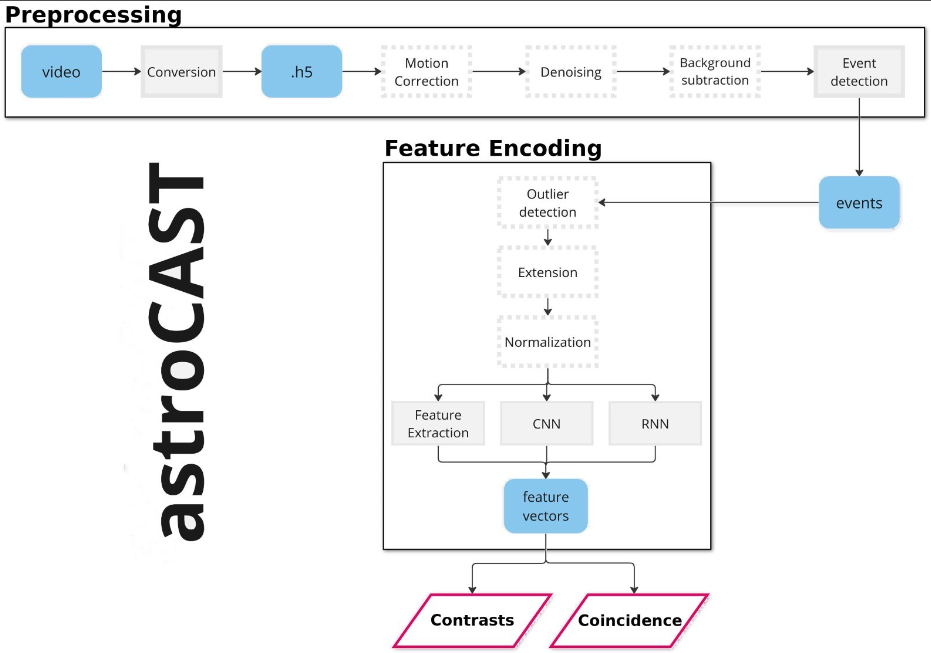
\includegraphics[width=\linewidth]{figures/1.png}
\end{center}
\caption{Schematic representation of the astroCAST toolkit comprising three major analytical phases for processing and analyzing astrocytic activity data. 1) In the preprocessing phase, video input is converted into an HDF5 file format, with optional stages for motion artifact correction, noise reduction, and background subtraction. 2) The event extraction phase involves the identification of astrocytic events, generating corresponding event traces and metadata. Events can subsequently undergo optional filtering, frame extension, and signal normalization. 3) The analysis of experiments is two-fold. For classification and regression, users may select from various feature vector embeddings including Feature Extraction (FExt), Convolutional Neural Network (CNN), and Recurrent Neural Network (RNN). For hierarchical clustering, the toolkit offers Pearson correlation and Dynamic Time Warping (DTW) for the computation of event similarity, represented as a distance matrix. Dashed outlines denote optional steps within the process. The presence of an open eye icon signifies supervised steps, while a closed eye indicates unsupervised steps. A line terminating in a circle denotes need for additional user input.}\label{fig:1}
\end{figure}

\begin{figure}[!htb]
\begin{center}
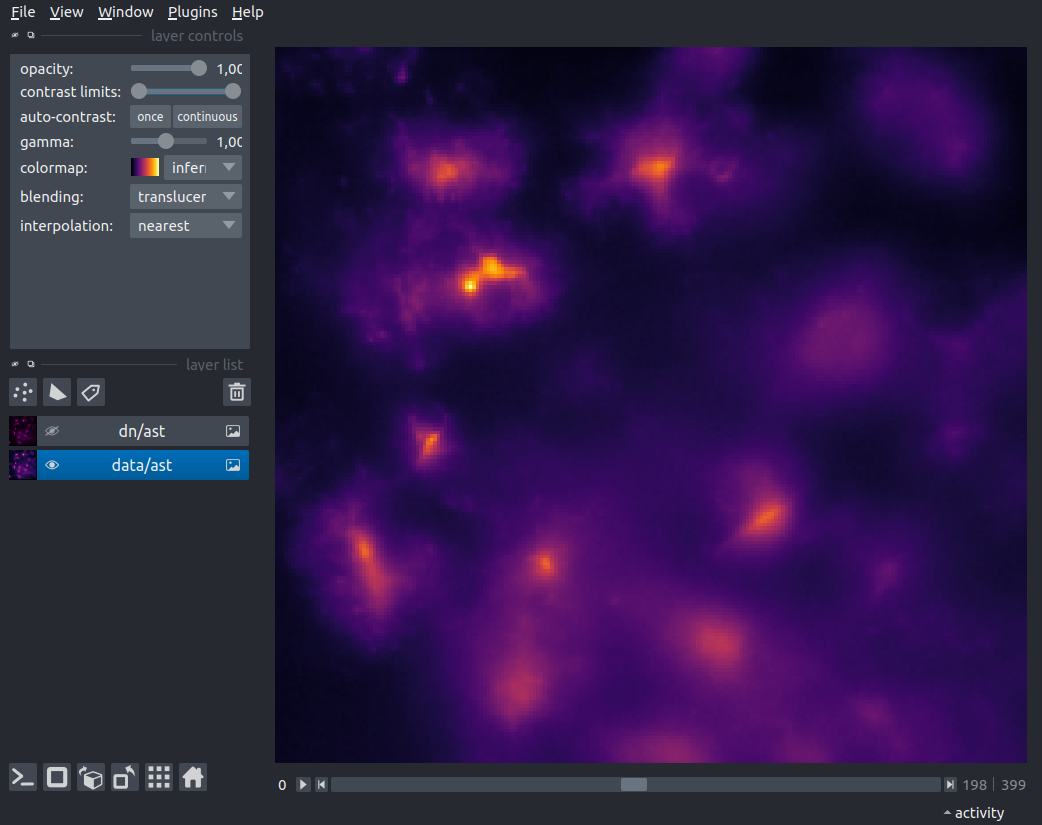
\includegraphics[width=\linewidth]{figures/2.png}
\end{center}
\caption{ The Astrocast Viewer interface, showcasing a video file of astrocytic calcium fluorescence captured within the inspiratory rhythm generator (preBötC) in the medulla. The original recording, acquired at a 20X magnification with a resolution of 1200x1200 pixels, was performed at a temporal resolution of 8Hz. The TIFF-format video was subsequently converted to the HDF5 file format, with spatial downscaling by a factor of four in the XY plane, as a preparatory step for further preprocessing.}\label{fig:2}
\end{figure}

\begin{figure}[!htb]
\begin{center}
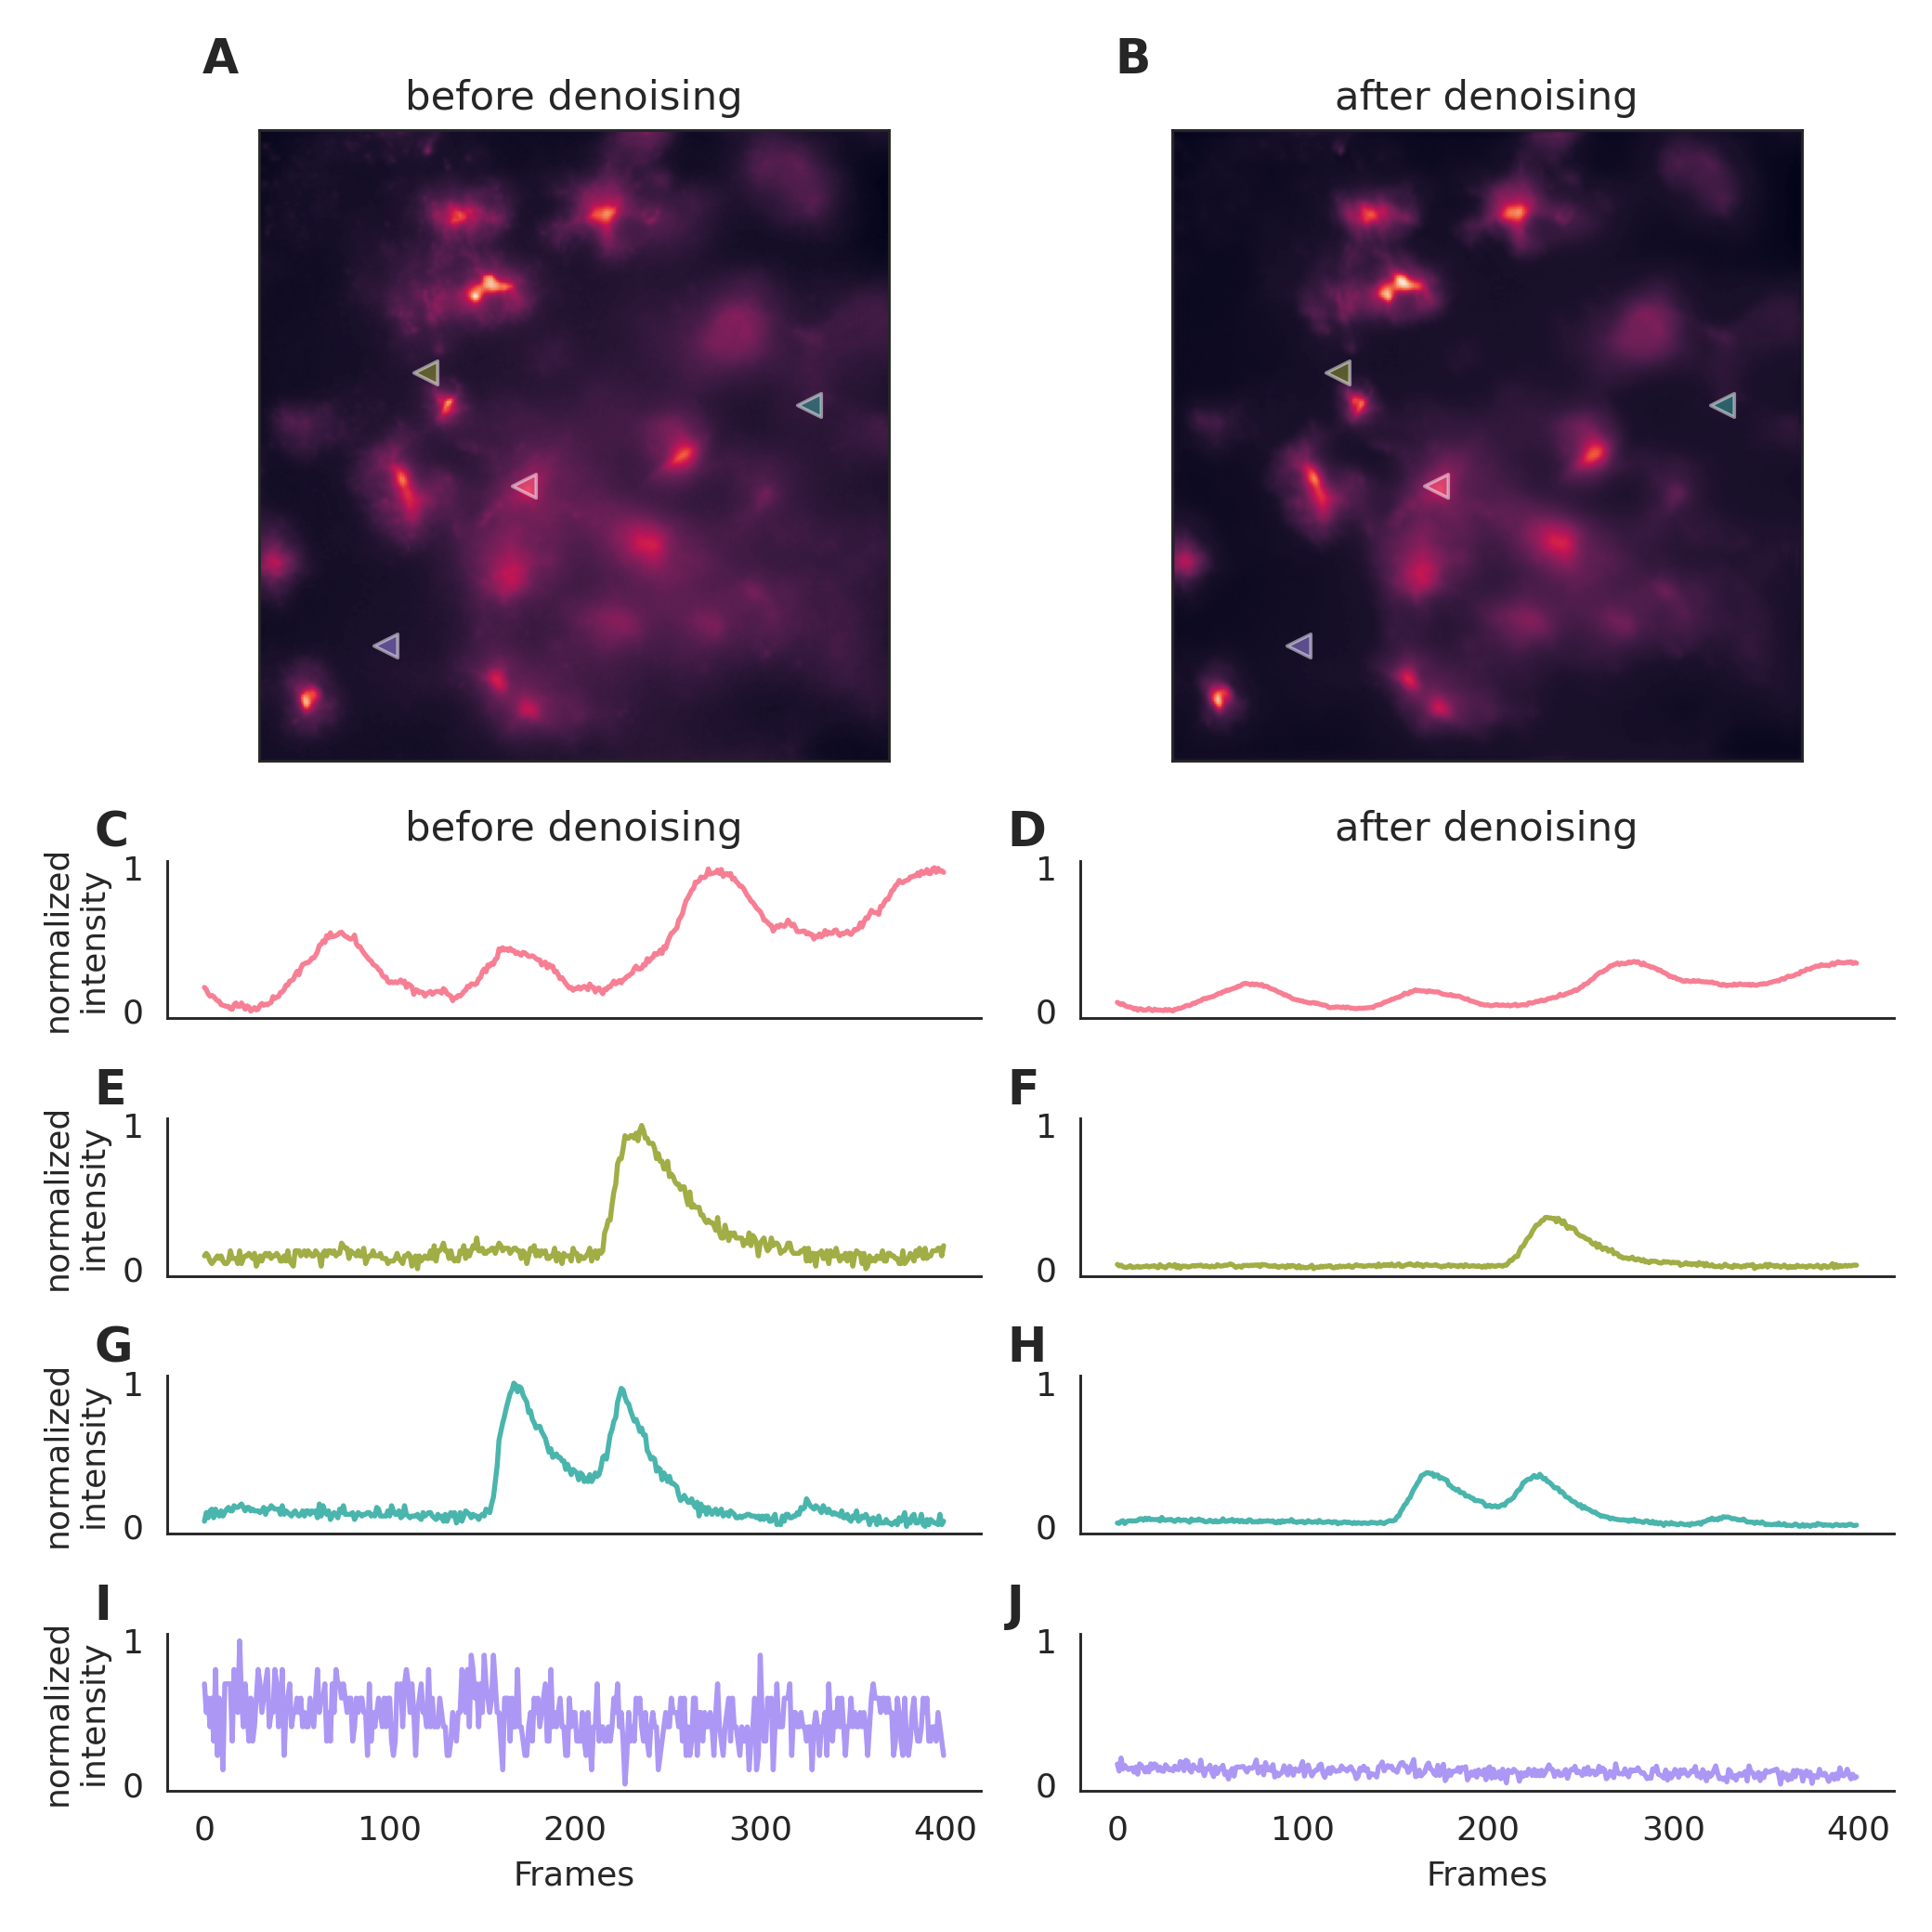
\includegraphics[width=\linewidth]{figures/3.png}
\end{center}
\caption{
Effect of denoising on astrocytic calcium imaging data. \textbf{(A)} A single 256x256 pixel frame prior to denoising, where background noise is evident. \textbf{(B)} The same frame following denoising with enhanced clarity. (C, E, G, and I) Pixel intensity over 400 frames (50s) before the application of the denoising algorithm, showcasing the original signal variation, after normalization. (D, F, H, J) Corresponding traces after denoising, illustrating a stabilized intensity profile, with preserved signal characteristics. The same normalization parameters were applied to both original and denoised traces to ensure comparability of noise levels. Location of pixels are indicated with triangles in A and B. The denoising algorithm was executed on a (128, 128) field of view, incorporating a context of five adjacent frames for each target frame, with no gap frames. Parameters for the denoising model included a training period of 50 epochs, a learning rate of 0.0001, momentum of 0.9, and a stack of three layers with 64 kernels of size three in the initial layer, omitting batch normalization. During inference, a strategy of a 10-pixel overlap in all directions, complemented by 'edge' padding, was employed. 
}\label{fig:3}
\end{figure}

\begin{figure}[!htb]
\begin{center}
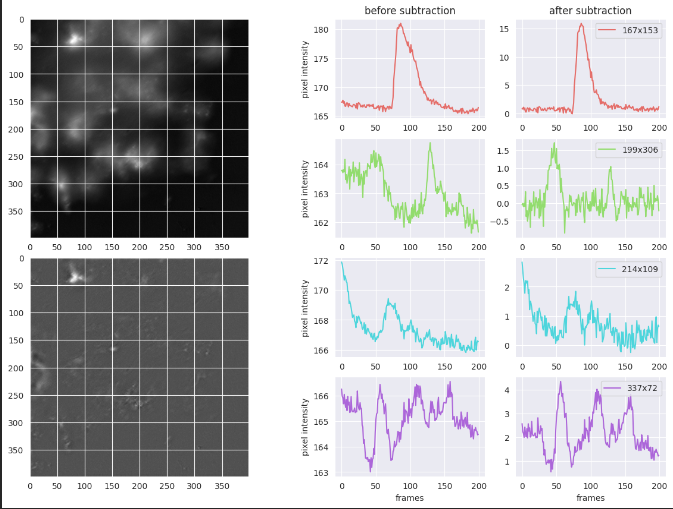
\includegraphics[width=\linewidth]{figures/4.png}
\end{center}
\caption{
Comparison before and after the application of background subtraction to fluorescence imaging data. (A, C) fluorescence images before and after background subtraction, respectively, illustrating the removal of extraneous noise. After subtraction, the background is close to zero and exhibits overall lower noise levels. (B, D) Intensity traces corresponding to the marked points on the images are plotted over time (400 frames, 50s). These traces highlight the efficacy of background subtraction, with the post-subtraction traces approaching zero on the y-axis, thereby indicating a substantial reduction of background, while signal amplitude is conserved. However, the signal shapes, especially in the red trace, exhibit slight alterations post-subtraction. Moreover, the green trace reveals the inadvertent introduction of spurious events, serving as a cautionary example of how background subtraction can inadvertently affect data integrity if parameters are not judiciously optimized.
}\label{fig:4}
\end{figure}

\begin{figure}[!htb]
\begin{center}
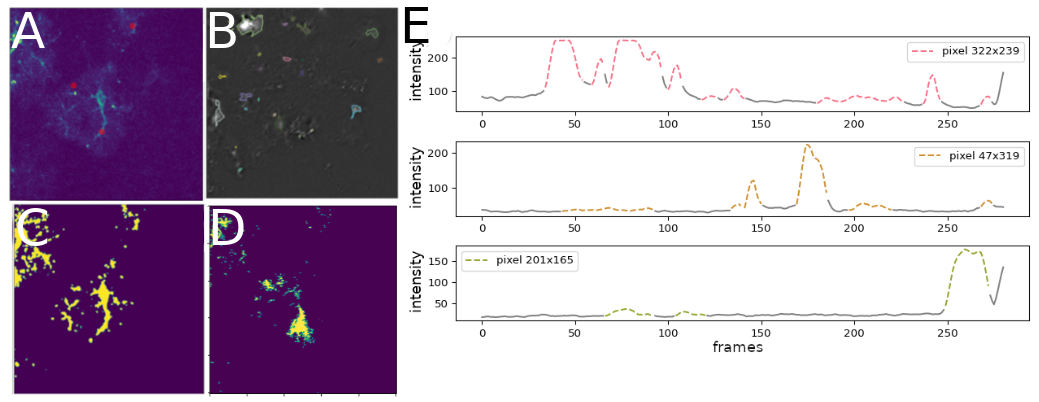
\includegraphics[width=\linewidth]{figures/5.png}
\end{center}
\caption{
Depiction of astrocytic event detection employed by astroCAST using spatial and temporal thresholding. A) Binary mask of frame after application of spatial threshold (min\_ratio 1). B) Binary mask of framer after application of temporal threshold (prominence 2, width 3, rel\_height 0.9). C) Frame used for thresholding after motion correction, denoising and smoothing. D) Events detected as identified by both spatial and temporal thresholding. E-G) Pixel intensity analysis for selected pixels (as indicated in Panels A-D), with active frames color-coded in the plots. The frame shown in A-D is indicated as a vertical dotted line.
}\label{fig:5}
\end{figure}

\begin{figure}[!htb]
\begin{center}
\includegraphics[width=\linewidth]{figures/6.png}
\end{center}
\caption{
Performance of Different Algorithms on Analyzing Various Synthetic Datasets. A) Showcase of synthetic calcium events designed to represent various levels of analytical difficulty, where color coding corresponds to events generated under different parameter sets that simulate diverse conditions or event types. All events include a random noise amplitude of 0.001 and parameter fluctuations of 0.01, subtly varying each event's parameters. B) Conditional contrasts analysis assesses algorithmic efficiency in distinguishing events from differing conditions (groups 0, 1 and 2). Events are characterized using different methods: FExt for Feature Extraction, CNN for Convolutional Autoencoder, and RNN for Recurrent Autoencoder. The hierarchical clustering leverages distance metrics between events (Pearson correlation or dynamic time warping), depicted by the absence of training dependency in grey. CNN's inability to process variable-length events results in its omission in the final panel. C) Coincidence detection analysis gauges algorithm performance in predicting the occurrence of stimulus events. This encompasses two groups: one with events exclusively occurring during a stimulus and another with randomly occurring events. The embedding classifier and prediction methods are consistent with panel B, where the classifier identifies stimulus occurrence, and regression determines the exact timing of the stimulus in coinciding events. \added[id=R2]{Displayed scores represent the lowest achieved in three replicates, adhering to cross-validation principles}.
}\label{fig:6}
\end{figure}

